\documentclass[a4paper,twoside,11pt,twocolumn]{article}

\usepackage[utf8]{inputenc}
\usepackage[T1]{fontenc}
\usepackage{textcomp}
\usepackage[english]{babel}
\usepackage{amsmath, amssymb, amsfonts, amsthm}
\usepackage{mathtools}
\usepackage{thmtools}
\usepackage{fancyhdr}
\pagestyle{fancy}
\fancyhf{}
\fancyhead[LE,RO]{Optimization for Machine Learning}
\fancyhead[RE,LO]{Notes and summary}
\fancyfoot[CE,CO]{\leftmark}
\fancyfoot[LE,RO]{\thepage}
\renewcommand{\headrulewidth}{2pt}
\renewcommand{\footrulewidth}{1pt}

% figure support
\usepackage{import}
\usepackage{xifthen}
\pdfminorversion=7
\usepackage{pdfpages}
\usepackage{transparent}
\newcommand{\incfig}[1]{%
	\def\svgwidth{0.8\columnwidth}
	\import{./figures/}{#1.pdf_tex}
}


% Define defentry
\makeatletter
\newif\ifdefentrybegin
\newcounter{defentry}[section]
\renewcommand{\thedefentry}{}
\newcommand{\defentry}{\@ifnextchar\begin\xnew@defentry\new@defentry}
\newcommand{\new@defentry}[1][]{%
  \par\addvspace{\topsep}%
  \refstepcounter{defentry}%
  \global\defentrybeginfalse
  \noindent\formatdefentry{#1}%
}
\newcommand{\formatdefentry}[1]{%
		\makebox[\parindent][l]{\Large\color{red}\bfseries\thedefentry}%
		\if\relax\detokenize{#1}\relax\else\textbf{\underline{\large{#1}}}\ \fi
}
\newcommand{\xnew@defentry}{%
  \refstepcounter{defentry}%
  \global\defentrybegintrue
}
\newcommand\defentrynumberorindent{%
  \ifdefentrybegin
    \formatdefentry{}%
  \else
    \hspace*{\parindent}%
  \fi
  \global\defentrybeginfalse
}
\makeatother

%Theorem
\newtheorem*{theorem*}{Theorem}
\newtheorem*{lemma*}{Lemma}
\newtheorem*{definition*}{Definition}

%useful math symbols
\newcommand\N{\ensuremath{\mathbb{N}}}
\newcommand\R{\ensuremath{\mathbb{R}}}
\newcommand\Z{\ensuremath{\mathbb{Z}}}
\renewcommand\O{\ensuremath{\mathcal{O}}}
\newcommand\Q{\ensuremath{\mathbb{Q}}}
\newcommand\E{\ensuremath{\mathbb{E}}}
\newcommand\C{\ensuremath{\mathbb{C}}}
\newcommand\dom{\ensuremath{\mathbf{dom}}}

\DeclareMathOperator*{\argmax}{argmax}
\DeclareMathOperator*{\argmin}{argmin}
\DeclareMathOperator{\prox}{prox}
\DeclareMathOperator{\indic}{\mathbf{\iota}}

\begin{document}
\section{Convexity}

\defentry[Cauchy-Schwarz] $\|\mathbf{u}^\top \mathbf{u}\| \le |\mathbf{u}\| |\mathbf{v}| \to \frac{\mathbf{u}^\top \mathbf{v}}{\| \mathbf{u} \| \| \mathbf{v} \|} \in [-1,1] \sim \cos\alpha$
\defentry[Definition of convexity] A function $f: \R^d \to \R$ is convex if (i) $\dom(f)$ is a convex set and (ii) $\forall \mathbf{x},\mathbf{y} \in \dom(f)$ and $\lambda\in \left[ 0,1 \right]$ we have \[\underbrace{f\left( \lambda x + (1-\lambda) y \right)}_{(1)} \leq \underbrace{\lambda f(x) + (1-\lambda)f(y)}_{(2)}\]
\begin{figure}[htpb]
	\centering
	\incfig{fig1}
	\caption{Any point on the line is above $f$}
	\label{fig:convexity_def}
\end{figure}
\defentry[Epigraph] While the \textit{graph} of a function is the line drawn by its expression, the \textit{epigraph} is the set of points that lie above the graph (the ``content'' of the graph).
\defentry[Jensen's inequality] The above definition is valid for any number of points in $\dom(f)$. Any ``middle point'' will be in-between them, and always above $f$. Formally: Let $f$ be convex, and $x_1,\ldots,x_m \in \dom(f),\ \lambda_1,\ldots,\lambda_m \in \R_+$ such that $\sum_{i=1}^{m}\lambda_i = 1 $. Then \[
	f\left( \sum_{i=1}^{m} \lambda_i \mathbf{x}_i  \right) \leq \sum_{i=1}^{m} \lambda_i f(\mathbf{x}_i)
	.\]
\defentry[Convex is continuous] Let f be convex, and suppose that $\dom(f)$ is open. Then $f$ is continuous. is continuous.
\defentry[Differentiable] Graph of the affine function $f(\mathbf{x}) + \nabla f(\mathbf{x})^\top(\mathbf{y}-\mathbf{x})$ is a tangent hyperplane to the graph of $f$ at $(\mathbf{x}, f(\mathbf{x})$
\defentry[First-order characterization] Suppose $\dom(f)$ is open and $f(\mathbf{x})$ is differentiable, in particular the gradient exists at every point $\mathbf{x} \in \dom(f)$. Then $f$ is convex if and only if $\dom(f)$ is convex and \[
	f(\mathbf{y}) \geq f(\mathbf{x}) + \nabla f(\mathbf{x})^\top (\mathbf{y}-\mathbf{x})
\]
This means that $f$ is above all its tangent hyperplanes.
\defentry[Second-order Characterization] Suppose that $\dom(f)$ is open, and that the Hessian (double derivatives) of $f$ exists at every point $\mathbf{x} \in \dom(f)$ and is symmetric. Then $f$ is convex if and only if $\dom(f)$ is convex, and for all $\mathbf{x} \in \dom(f)$ we have
\[
	\nabla^2 f(\mathbf{x}) \succeq 0\footnote{positive semidefinite}
\]

\defentry[Operations] Multiplication by real constant and addition between convex is convex (not everywhere, only on $\bigcap_{i=1}^m \dom(f_i)$). The composition works the following: Let $f$ be a convex function with $\dom(f) \subseteq \R^d,\ g: \R^m \to \R^d$ an affine function, meaning that $g(\mathbf{x}) = A\mathbf{x} + \mathbf{b}$, for some matrix $A \in \R^{d\times m}$ and some vector $\mathbf{b} \in  \R^d$. Then the function $f \circ g$ (that maps $\mathbf{x}$ to $f(A\mathbf{x} + \mathbf{b})$ is convex on $\dom(f \circ g) := \left\{ \mathbf{x} \in \R^m: g(\mathbf{x}) \in \dom(f) \right\} $

\defentry[Mimima] $\mathbf{x}$ is a local minimum if $\exists \epsilon > 0$ with \[
	f(\mathbf{x}) \leq f(\mathbf{y})
\]
For all $\mathbf{y} \in  \dom(f)$ satisfying $\|\mathbf{y}-\mathbf{x}\| < \epsilon$. If $\mathbf{x}^\star$ is the local minimum of a convex function, then it's a global minimum (meaning $f(\mathbf{x}^\star) \leq f(\mathbf{y})$ for all $\mathbf{y} \in \dom(f)$.
Similarly, for $f$ convex and differentiable over an open domain, then if $\nabla f(\mathbf{x}) = \mathbf{0}$ then it's a global minimum (it's called a \textit{critical point}).

\defentry[Strictly convex] Same definition as the convexity, with a strict inequality. So the open segment connecting any two points of the graph will be \textit{strictly} above the graph. This leads to the following lemma:
\begin{lemma*}
	Suppose that $\dom(f)$ is open and that $f$ is twice continuously differentiable. If the Hessian $\nabla^2 f(\mathbf{x}) \succeq \mathbf{0}$ for every $\mathbf{x} \in \dom(f)$, then f is strictly convex.
\end{lemma*}

\defentry[Constrained] Let $f: \dom(f) \to \R$ be convex, and let $X \subseteq \dom(f)$ be a convex set. A point $\mathbf{x} \in X$ is a \textit{minimizer of $f$ over $X$} if $f(\mathbf{x}) \le f(\mathbf{y})\ \forall \mathbf{y} \in X$. It follows that for $f: \dom(f) \to  \R$ convex and differentiable oven an open domain $\dom(f) \subseteq \R^d$, and for $X \subseteq$ a convex set, then the point $\mathbf{x}^\star \in X$ is a minimizer of $f$ over $X$ iff \[
	\nabla f(\mathbf{x}^\star)^\top(\mathbf{x}-\mathbf{x}^\star) \ge 0\ \forall \mathbf{x}\in X
\]
\defentry[$\alpha$-sublevel] $f^{\leq \alpha} := \{\mathbf{x} \in  \R^d : f(\mathbf{x}) \leq \alpha$. This represents the values of the domain of $f$ for which the value of $f$ is below a threshold
\begin{figure}[htpb]
	\centering
	\incfig{fig2}
	\caption{Only what is between vertical bars is in the sublevel}
	\label{fig:sublevel}
\end{figure}
\defentry[Weierstrass theorem] Let $f: \R^d \to \R$ be a convex function, and suppose there is a nonempty and bounded sublevel set $f^{\le \alpha}$. Then f has a global minimum. Some function (such as $e^x$) don't have a minimum (in the exponential case, because the subvlevel is not bounded.


\section{Gradient descent}
\defentry[Gradient descent] \underline{Goal}: get near to a minimum  $x^\star$ (not necessarily unique), meaning close to the optimal value $f(x^\star)$. For that, we look for $\mathbf{x} \in  \R^d$ such that
\[
	f(\mathbf{x}) - f(\mathbf{x}^\star) \leq \epsilon
\]
\underline{Iterative algorithm:} For that purpose, we start from $\mathbf{x}_0 \in  \R^d$, and then iterate: \[
	\mathbf{x}_{t+1} :=\mathbf{x}_t - \gamma \nabla f(\mathbf{x}_t)
\]
For time steps t=0,1,\ldots, and step size $\gamma \geq 0$

\defentry[Bound to error (vanilla)] It's useful to bound the error ($f(\mathbf{x}_t) - f(\mathbf{x}^\star)$). Using the notation $\mathbf{g}_t := \nabla f(\mathbf{x}_t)$ (for gradient descent, $\mathbf{g}_t = \frac{\mathbf{x}_t - \mathbf{x}_{t+1}}{\gamma}$ ), and applying the following steps:
\begin{enumerate}
	\item Apply $2\mathbf{v}^\top \mathbf{w} = \|\mathbf{v}\|^2 + \|\mathbf{w}\|^2 - \|\mathbf{v}-\mathbf{w}\|^2$
	\item Sum over for the first $T$ iterations
	\item Use first-order characterization with $\mathbf{x} = \mathbf{x}_t,\mathbf{y}=\mathbf{x}^\star$.
\end{enumerate}
We obtain the upper bound for the \underline{average error}: \[
	\sum_{t=0}^{T-1}\left( f(\mathbf{x}_t) - f(\mathbf{x}^\star) \right) \leq \frac{\gamma}{2}
	\sum_{t=0}^{T-1} \|\mathbf{g}_t\|^2 + \frac{1}{2\gamma} \|\mathbf{x}_0 - \mathbf{x}^\star\|^2 \]

\defentry[Lipschitz]
\begin{theorem*}
	A function $f: \dom(f) \to \R^m$ is \textit{B-Lipschitz} if \[
		\|f(\mathbf{x}) - f(\mathbf{y})\| \leq B\|\mathbf{x}-\mathbf{y}\|
	\] for all $\mathbf{x},\mathbf{y} \in \dom(f)$
\end{theorem*}
Assume all gradients of $f$ bounded in norm (not always cool, e.g. discards $x^2$). The following theorem holds:
\begin{theorem*}
	Let $f: \R^d \to  \R$ be convex and differentiable, and suppose $\|\mathbf{x}_0 - \mathbf{x}^\star\| \leq R$, and $\|\nabla f(\mathbf{x})\| \leq B$ for all $\mathbf{x}$. Choosing the step size \[
		\gamma := \frac{R}{B\sqrt{T}}
	\] then gradient descent yields \[
		\frac{1}{T}\sum_{t=0}^{T-1}f(\mathbf{x}_t) - f(\mathbf{x}^\star) \leq \frac{RB}{\sqrt{T} }
	\]
\end{theorem*}
This relates $T$ and $\epsilon$ ! \[
	T \geq \frac{R^2B^2}{\epsilon^2} \Rightarrow \text{average error } \leq \frac{RB}{\sqrt{T}} \leq \epsilon
\]
Note: same for subgradient descent.

\defentry[Smoothness] A function is smooth if it is ``Not too curved''. That is, if given a point $\mathbf{x} \in X$, all other points smaller than the linearisation + a quadratic term. Formally, let $f: \dom(f) \to \R$ be differentiable, $X \subset \dom(f),\ L \in \R_+$. $f$ is called smooth (with parameter $L$ over $X$ if
\[
	f(\mathbf{y}) \leq f(\mathbf{x}) + \nabla f(\mathbf{x})^\top (\mathbf{y}-\mathbf{x})+\frac{L}{2} \|\mathbf{x}-\mathbf{y}\|^2
\] $\forall \mathbf{x},\mathbf{y} \in X$.

\begin{figure}[htpb]
	\centering
	\incfig{fig3}
	\caption{Every $\mathbf{y}$ is below the linearisation+quadratic}
	\label{fig:smooth_func}
\end{figure}

(unsure) The smoothness of least squares ($f(x) = \frac{1}{2n} \|A\mathbf{x} + \mathbf{b}\|$ ) is given by $\max\frac{\|A^\top \cdot A\|}{n}$. That is the maximum of the eigenvalues of $A^\top \cdot A$ divided by the number of rows of $A$.
\defentry[Operations on Smoothness]	Addition of smooth function is still smooth: $f_1, f_2,\ldots,f_m$ smooth with parameters $L_1,L_2,\ldots,L_m$ and let $\lambda_1, \lambda_2,\ldots,\lambda_m \in  \R_+$. Then $f := \sum_{i=1}^{m} \lambda_i L_i $ is smooth, with parameter $\sum_{i=1}^{m} \lambda_i L_i $.

Also, about composition: $f$ $L$-smooth, and let $g(\mathbf{x}) = A\mathbf{x} + \mathbf{b}$ for $A \in  \R^{d \times m},\ \mathbf{b} \in  \R^d$. Then $f \circ g$ is smooth with parameter $L\|A\|^2$ (where $\|A\|$ is the spectral norm of $A$).

\defentry[Smooth VS Lipschitz]
\begin{enumerate}
	\item Bounded gradients $\iff$ Lipschitz continuity of $f$
	\item Smoothness $\iff$ Lipschitz continuity of $\nabla f$
\end{enumerate}
For $f: \R^d \to  \R$, convex and differentiable, the following are equivalent:
\begin{itemize}
	\item $f$ is smooth with parameter $L$
	\item $\|\nabla f(\mathbf{x}) - \nabla f(\mathbf{y})\| \leq L \|\mathbf{x}-\mathbf{y}\|$ for all $\mathbf{x},\mathbf{y} \in  \R^d$
\end{itemize}

\defentry[Sufficient decrease] $f: \R^{d} \to \R$ differentiable, $L$-smooth, step size $\gamma := \frac{1}{L}$. Then gradient descent satisfies \[
	f(\mathbf{x}_{t+1}) \leq f(\mathbf{x}_t) - \frac{1}{2L}\|\nabla f(\mathbf{x}_t)\|^2\quad t\geq 0
\]
This is a strong statement. This implies that the steps always get better (second term is always positive)
\defentry[Smooth \& convex] $f$ convex, differentiable, with global minimum, $L$-smooth, step size $\frac{1}{L}$. Gradient descent yields \[
	f(\mathbf{x}_t) - f(\mathbf{x}^\star) \leq \frac{L}{2T} \|\mathbf{x}_0 - \mathbf{x}^\star\|^2,\ T>0
\]
This relates $T$ and $\epsilon$ ! \[
	T > \frac{R^2L}{2\epsilon} \Rightarrow \text{error} \leq \frac{L}{2T} \leq \epsilon
\]

\defentry[Strongly convex] Up until now, error decreased in $T$ or $\sqrt{T}$. Good, but not ideal. Strongly convex functions converge exponentially. For $f: \dom(f) \to \R$ differentiable function, $X \subset \dom(f)$ convex and $\mu \in  \R_+,\ \mu > 0$. Then $f$ is strongly convex (with parameter $\mu$) over $X$ if
\begin{align*}
	f(\mathbf{y}) \geq & \overbrace{f(\mathbf{x}) + \nabla f(\mathbf{x})^\top(\mathbf{y}-\mathbf{x})}^{\text{Linearisation at } x}                \\
	                   & + \underbrace{\frac{\mu}{2}\|\mathbf{x}-\mathbf{y}\|^2}_{\text{Quadratic term}}\quad \forall \mathbf{x},\mathbf{y} \in X
\end{align*}
\begin{figure}[htpb]
	\centering
	\incfig{fig4}
	\caption{Function is between smooth (above) and strongly convex (below)}
	\label{fig:strongly_convex}
\end{figure}

\defentry[Smooth \& Strongly convex] We start from the vanilla analysis, and use stronger lower bound on left-hand side (coming from strong convexity). That is, we use that \[
	\nabla f(\mathbf{x}_t)^\top (\mathbf{x}_t - \mathbf{x}^\star) \geq f(\mathbf{x}_t) -f(\mathbf{x}^\star) + \frac{\mu}{2} \|\mathbf{x}_t - \mathbf{x}^\star\|^2
\]
and some rewriting to obtain the final bound:
\begin{align*}
	\|\mathbf{x}_{t+1} - \mathbf{x}^\star\|^2 \leq & 2\gamma\left( f(\mathbf{x}^\star) - f(\mathbf{x}_t) \right) \\
	                                               & + \gamma^2 \|\nabla f(\mathbf{x}_t)\|                       \\
	                                               & + (1-\mu\gamma)\|\mathbf{x}_t - \mathbf{x}^\star\|^2
\end{align*}
In other words: \textit{Squared distance to $\mathbf{x}^\star$ goes down by a constant factor, up to some ``noise''}. This leads to the following theorem:
\begin{theorem*}
	Let $f: \R^{d} \to \R$, differentiable, with a global minimum $x^\star$. Suppose it's smooth with parameter $L$ and strongly convex with parameter $\mu > 0$. With $\gamma := \frac{1}{L}$, gradient descent with arbitrary $\mathbf{x}_0$ satisfies the following 2 properties:
	\begin{itemize}
		\item Squared distance to $\mathbf{x}^\star$ are geometrically decreasing: \[
			      \|\mathbf{x}_{t+1} - \mathbf{x}^\star\|^2 \leq \left( 1-\frac{\mu}{L} \right) \|\mathbf{x}_t - \mathbf{x}^\star\|^2,\ t \geq 0
		      \]
		\item The absolute error after $T$ iterations is exponentially small in $T$ : \[
			      f(\mathbf{x}_T) - f(\mathbf{x}^\star) \leq \frac{L}{2}\left( 1-\frac{\mu}{L})\right)^{T} \|\mathbf{x}_0 - \mathbf{x}^\star\|^2
		      \]
	\end{itemize}
\end{theorem*}

\section{Projected Gradient Descent}
\defentry[Constrained Optimization] We want to minimize $f(\mathbf{x})$, but being subject to $\mathbf{x} \in X$. 2 ways of solving this: Either use projected gradient descent, or transform it into an \textit{unconstrained} problem.
\defentry[Projected Gradient Descent] Idea: project onto $X$ after every step:
\[
	\Pi_X(\mathbf{y}) := \argmin_{\mathbf{x} \in  X} \|\mathbf{x}-\mathbf{y}\|
\]
Idea: compute first what would be your next step ($\mathbf{y}_{t+1}$) and then project it on your actual next step. \[
	\begin{array}{lll}
		\mathbf{y}_{t+1} & := & \mathbf{x}_{t} - \gamma \nabla  f(\mathbf{x}_t),                                        \\
		\mathbf{x}_{t+1} & := & \Pi_X(\mathbf{y}_{t+1}) := \argmin_{\mathbf{x} \in X} \|\mathbf{x}-\mathbf{y}_{t+1}\|^2
	\end{array}
\]
\defentry[Properties] Let $X \in  \R^d$ be closed and convex, $\mathbf{x} \in  X, \mathbf{y} \in  \R^d$. Then
\begin{itemize}
	\item  $\left(\mathbf{x} - \Pi_X(\mathbf{y})\right)^\top (\mathbf{y}-\Pi_X(\mathbf{y})) \leq 0$
	\item $\|\mathbf{x} - \Pi_X(\mathbf{y})\|^2 + \|\mathbf{y}-\Pi_X(\mathbf{y})\|^2 \leq \|\mathbf{x}-\mathbf{y}\|^2$
\end{itemize}
First property means that for any point $\mathbf{y}$, and any point $\mathbf{x}$ in the domain, then the angle formed at the projection of $\mathbf{y}$ (in $X$ ) is greater than $90^\circ$ (negative inner product).

Second property is the triangle inequality: distance $x$-projection plus projection-$\mathbf{y}$ is bigger than distance $\mathbf{x}-\mathbf{y}$. Inequality is written in the other round because of the squared values. If you remove the square, then inequality reverts.

Last cool property: The expected number of steps in various scenarios (Lipschitz,\ldots), as listed in appendix Table \ref{tab:convergence_speed}, remains unchanged!

\defentry[Equivalent proofs of projected] The last property abode needs to be proved (not here). However, here are some insights: We now only need the function to be continuous over $X$, and not anymore $\R^d$. Then, in the proofs we replace $\mathbf{x}_{_t+1}$ by  $\mathbf{y}_{t+1}$, and massage it with the facts above.

\defentry[Smooth and strongly convex over $X$]
\begin{theorem*}
	Let $f: \R^d \to  \R$ be convex and differentiable. Let $D \subseteq \R^d$ be a normal nonempty closed and convex set and suppose that $f$ is smooth over $X$ with parameter $L$ and strongly convex over $X$ with parameter $\mu > 0$. Choosing $\gamma := \frac{1}{L}$, \textbf{projected} gradient descent with arbitrary $\mathbf{x}_0$ satisfies the following two properties:
	\begin{enumerate}
		\item Squared distance to $\mathbf{x}^\star$ are geometrically decreasing: \[
			      \|\mathbf{x}_{t+1} - \mathbf{x}^\star\|^2 \le \left( 1- \frac{\mu}{L} \right) \|\mathbf{x}_t - \mathbf{x}^\star\|^2,\ t \ge 0
		      \]
		\item The absolute error after $T$ iterations is exponentially small in $T $: \[
			      \begin{array}{l}
				      f(\mathbf{x}_T) - f(\mathbf{x}^\star) \\ \le  \|\nabla f(\mathbf{x}^\star)\| \left( 1- \frac{\mu}{L} \right)^{T/2} \|\mathbf{x}_{0} - \mathbf{x}^\star\|\\

				      + \frac{L}{2}\left( 1-\frac{\mu}{L}\right)^\top \|\mathbf{x}_0 - \mathbf{x}^\star\|
			      \end{array}
		      \]
	\end{enumerate}
\end{theorem*}

\defentry[Projection step] Computing the projection is far from obvious. But for some relevant cases, it can be efficiently solved:
\begin{itemize}
	\item Projecting onto an affine subspace (leads to system of linear equations)
	\item Projecting onto an Euclidean ball with center $\mathbf{c}$ (scale vector $\mathbf{y}-\mathbf{c})$. Compute $y = (\mathbf{y}-\mathbf{c})\cdot \frac{R}{\|\mathbf{x}\|}$.
	\item Projecting onto $\ell_1$-balls (needed in Lasso). Though, we restrict to the ball being centered at $\mathbf{0}$, defined as \[
		      B_1(R) = \left\{ \mathbf{x}\in \R^d : \|\mathbf{x}\|_1 = \sum_{i=1}^{d}|x_i| \leq R  \right\}
	      \]
	      $B_1$ is a \textit{cross polytope} ($2d$ facets, $2^d$ vertices). The projection can be computed in $\O(d \log d)$, and even improved to $\O(d)$
\end{itemize}

\section{Proximal and Subgradient Descent}
\defentry[Composite optimization problems] Consider $f(\mathbf{x}) := g(\mathbf{x}) + h(\mathbf{x})$, where $g$ is ``nice'' and $h$ is a ``simple'' additional term (but not nice). Important case when $h$ is not differentiable.
\defentry[Proximal gradient] Classical gradient step: \[
	\mathbf{x}_{t+1} = \argmin_\mathbf{y} g(\mathbf{x}_t)^\top (\mathbf{y}-\mathbf{x}_t) + \frac{1}{2\gamma}\|\mathbf{y}-\mathbf{x}_t\|^2
\] For $f = g+h$ keep the same for $g$ and add $h$ unmodified:\[
	\begin{array}{ll}
		\mathbf{x}_{t+1} & = \overbrace{\argmin\limits_\mathbf{y} g(\mathbf{x}_t)^\top (\mathbf{y}-\mathbf{x}_t) + \frac{1}{2\gamma}\|\mathbf{y}-\mathbf{x}_t\|^2}^{\text{Quadratic upperbound from smooth }g} + \overbrace{h(\mathbf{y})}^{\text{Non smooth}} \\
		                 & = \argmin\limits_{\mathbf{y}} \frac{1}{2\gamma} \|\mathbf{y}-(\mathbf{x}_t - \gamma \nabla g(\mathbf{x}_t))\|^2 + h(\mathbf{y})
	\end{array}
\]
The name comes because you can rewrite it using the \textit{proximal} operator.
\defentry[Proximal mapping] We define the proximal mapping as follow: for a given $h$ and a $\gamma > 0$ : \[
	\prox_{h,\gamma}(\mathbf{z}) := \argmin_\mathbf{y} \left\{ \frac{1}{2\gamma} \|\mathbf{y}-\mathbf{z}^2 + h(\mathbf{y}\| \right\}
\]
Using the above definition, one iteration of proximal gradient descent can be rewritten as \[
	\mathbf{x}_{t+1} := \prox_{h,\gamma}(\mathbf{x} - \gamma \nabla g(\mathbf{x}_t))
\]
\defentry[Generalized gradient] The above allows us to describe the generalized gradient as \[
	G_{h,\gamma} := \frac{1}{\gamma}\left( \mathbf{x} - \prox_{h,\gamma}(\mathbf{x}-\gamma \nabla g(\mathbf{x}))) \right)
\]  and thus rewrite the update step as \[
	\mathbf{x}_{t+1} = \mathbf{x}_{t} - \gamma G_\gamma(\mathbf{x}_t)
\]
\defentry[Generalization] Proximal is generalization of gradient descent. If $h$ is 0, it's gradient descent, if it's $\indic_X$, it's the projected gradient descend. With \[
	\indic_{X}(\mathbf{x}) := \left\{ \begin{array}{ll}
		0       & \text{if } \mathbf{x} \in X \\
		+\infty & \text{otherwise}
	\end{array}\right.
\] Proximal mapping becomes, with $\indic_X$ it becomes $\prox_{h,\gamma} = \argmin_{\mathbf{y}\in  X} \|\mathbf{y}-\mathbf{z}\|^2$

\defentry[Convergence] $\O(\frac{1}{\epsilon})$ for smooth (same as vanilla), and if also strongly convex $\O(\log(\frac{1}{\epsilon}))$. Same as vanilla case for smooth functions, but now for any $h$ \textit{for which we can compute the proximal mapping}
\defentry[Subgradient] $\mathbf{g} \in \R^d$ is a subgradient of $f$ at  $\mathbf{x}$ if \[
	f(\mathbf{y}) \geq \mathbf{g}^\top(\mathbf{y}-\mathbf{x})\ \forall \mathbf{y} \in \dom(f)
\]
\defentry[Subdifferential] $\partial f(\mathbf{x}) \subseteq \R^d$ is the set of subgradients of $f$ at $\mathbf{x}$.
\begin{lemma*}
	If $f: \dom(f) \to \R$ is differentiable at $\mathbf{x} \in  \dom(f)$, then $\partial f(\mathbf{x}) \subseteq \left\{ \nabla f(\mathbf{x}) \right\} $
\end{lemma*}
This means at differentiable points of a function, there is either exactly one subgradient (that is the true gradient) or no subgradient at all (because it's a gradient, but above, in case of non-convex)
\defentry[Subgradient and convexity] ``Convex = subgradients everywhere''.
\begin{lemma*}
	Let $f: \dom(f) \to  \R$ is convex if and only if $\dom(f)$ is convex and $\partial f(\mathbf{x}) \neq \emptyset$ $\forall \mathbf{x} \in  \dom(f)$
\end{lemma*}
\defentry[Convex and Lipschitz]
Convex and Lipschitz = bounded subgradient.
\begin{lemma*}
	Let $f: \dom(f) \to  \R$ convex, $\dom(f)$ open, $B \in  \R_+$. Then the following are equivalent:
	\begin{itemize}
		\item $\|\mathbf{g}\| \le B\ \forall \mathbf{x} \in \dom(f),\ \forall \mathbf{g} \in  \partial f(\mathbf{x})$.
		\item $|f(\mathbf{x}) - f(\mathbf{y})| \le B\|\mathbf{x}-\mathbf{y}\|\ \forall \mathbf{x},\mathbf{y} \in \dom(f)$
	\end{itemize}
\end{lemma*}

\defentry[Subgradient optimality condition]
\begin{lemma*}
	Suppose $f: \dom(f) \to  \R$ and $\mathbf{x} \in \dom(f)$. If $\mathbf{0} \in \partial f(x)$, then $\mathbf{x}$ is a global minimum
\end{lemma*}
\defentry[Differentiability]
\begin{theorem*}
	A convex function $f: \dom(f) \to  \R$ is differentiable almost everywhere.
\end{theorem*}
Meaning: set of points where $f$ is non-differentiable has measure 0 (no volume), and for all $\mathbf{x} \in  \dom(f)$ and all $\epsilon > 0$, there is a point $\mathbf{x}'$ such that $\|\mathbf{x}-\mathbf{x}'\| < \epsilon$ and $f$ is differentiable at $\mathbf{x}'$. This is a problem for gradient descent. Min can be non-differentiable, and non-differentiable points can be requested during descent.

\defentry[Subgradient descent] To solve this: use subgradient descent. Choose starting point $\mathbf{x}_0 \in \R^d$. Then for each times $t=0,1,\ldots$ and stepsizes $\gamma_t \geq 0$ (not necessarily fixed) : \[
	\begin{array}{c}
		\text{Let } \mathbf{g}_t \in \partial f(\mathbf{x}_t) \\
		\mathbf{x}_{t+1} := \mathbf{x}_t - \gamma_t \mathbf{g}_t
	\end{array}
\]
\defentry[Optimality] Many convergence rates. Can we always improve? No.
\begin{theorem*}[Nesterov]
	For any $T \leq d-1$ and starting point $\mathbf{x}_0$, there is a function $f$ in the problem class of B-Lipschitz function over $\R^d$, such that any (sub)gradient method has an objective error at least \[
		f(\mathbf{x}_T) - f(\mathbf{x}^\star) \geq \frac{RB}{2(1+\sqrt{T+1})}
	\]
\end{theorem*}
This means that if we only have access to first order methods and the function is only Lipschitz, (no additional assumption), then the subgradient algorithm is optimal, and the convergence rate can't be faster than $\sim \frac{1}{\sqrt{T}}$.

\defentry[Smooth non-differentiable] If function is non-differentiable, it can't be smooth (so we can't use that assumption). Yet, we can still be better than $\O(\frac{1}{\epsilon^2})$ if we require strong convexity.

\defentry[Strongly convex] Definition is similar that for gradient, with the use of subgradient. \[
	f(\mathbf{y}) \geq \overbrace{f(\mathbf{x}) + \mathbf{g}^\top(\mathbf{y}-\mathbf{x})}^{\text{Linearisation at } x} + \underbrace{\frac{\mu}{2}\|\mathbf{x}-\mathbf{y}\|^2}_{\text{Quadratic term}}
\]
$\forall \mathbf{x},\mathbf{y} \in \dom(f), \forall \mathbf{g} \in \partial f(\mathbf{x})$. Alternatively:
\begin{lemma*}
	Let $f: \dom(f)\to \R$ be convex, $\dom(f)$ open, $\mu \in \R_+^*$. $f$ is strongly convex with parameter $\mu$ if and only if $f_\mu : \dom(f)\to \R$ defined by \[
		f_\mu(\mathbf{x}) = f(\mathbf{x}) - \frac{\mu}{2}\|\mathbf{x}\|^2,\ \mathbf{x}\in \dom(f)
	\] is convex
\end{lemma*}

\defentry[Tame strong convexity] Over $\R^d$, strong convexity and subgradients contradict each other. With strong convexity, gradients will explode to infinity.
\begin{theorem*}
	Let $f: \R^d \to  \R$ be strongly convex with parameter $\mu > 0$, and let $\mathbf{x}^\star$ be the unique global 	minimum of $f$. With decreasing step size \[
		\gamma_t := \frac{2}{\mu(t+1)},\ t>0
	\]
	subgradient descent yields \[
		\underbrace{f\left( \frac{2}{T(T+1)}\sum_{t=1}^{T} t\cdot \mathbf{x}_t  \right)}_{\text{convex combination of iterates}} - f(\mathbf{x}^\star) \leq \frac{2B^2}{\mu(T+1)}
	\] where $B = \max_{t=1}^{T} \|\mathbf{g}_t\|$
\end{theorem*}
\defentry[Strong convexity]
\section{Stochastic Gradient Descent}
\defentry[Idea] Many objective functions are sum structured \[
	f(\mathbf{x}) = \frac{1}{n}\sum_{i=1}^{n}f_i(\mathbf{x})
\]
As for example, $f_i$ is the cost function of $i$-th observation. But doing so on very large datasets (e.g. Imagenet, $n\simeq 14M$). So we only do on a subset.
\defentry[The algorithm] As always, get a starting point $\mathbf{x}_0 \in \R^d$, then sample $i \in  [n]$ uniformly at random, and compute as before: \[
	\mathbf{x}_{t+1} := \mathbf{x}_t - \gamma_t \nabla f_i(\mathbf{x}_t)
\]
So we only update with the gradient of $f_i$ instead of the full gradient. The vector $\mathbf{g}_t := \nabla f_i(\mathbf{x}_t)$ is called a stochastic gradient.
\defentry[Analysis] We can't use the same as vanilla, because convexity $\big(f(\mathbf{x}_t) - f(\mathbf{x}^\star) \leq \mathbf{g}_t^\top(\mathbf{x}_t - \mathbf{x}^\star)$\big) doesn't hold anymore. But cool thing! $\mathbf{g}_t$ is an unbiased estimate of the full gradient: \[
	\E[\mathbf{g}_t | \mathbf{x}_t = \mathbf{x}] = \frac{1}{n}\sum_{i=1}^{n}\nabla f_i(\mathbf{x}) = \nabla f(\mathbf{x})
\]
So the convexity inequality holds in expectation.

\defentry[Holds in expectation] For any fixed $\mathbf{x}$, linearity of conditional expectations yields \[
	\begin{array}{ll}
		  & \E\left[\mathbf{g}_t(\mathbf{x}-\mathbf{x}^\star) | \mathbf{x}_t = \mathbf{x}\right]       \\
		= & \E\left[\mathbf{g}_t | \mathbf{x}_t = \mathbf{x}\right]^\top (\mathbf{x}-\mathbf{x}^\star) \\
		= & \nabla f(\mathbf{x})^\top(\mathbf{x}-\mathbf{x}^\star)
	\end{array}
\]
\defentry[Bounded stochastic gradient]
\begin{theorem*}
	Let $f: \R^d \to  \R$ be convex and differentiable, $\mathbf{x}^\star$ a global minimum. Furthermore, suppose that $\|\mathbf{x}_0 - \mathbf{x}^\star\| \leq R$ and that $\E\left[\|\mathbf{g}_t\|^2\right] \leq B^2$ for all $t$. Choosing the constant stepsize \[
		\gamma := \frac{R}{B\sqrt{T} }
	\] stochastic gradient descent yields \[
		\frac{1}{T}\sum_{t=0}^{T-1}\E\left[f(\mathbf{x}_t)\right] - f(\mathbf{x}^\star) \leq \frac{RB}{\sqrt{T} }
	\]
\end{theorem*}
Note that in this theorem, the step size is constant.
\defentry[Convergence rate: SGD vs GD]
For GD: we assumed $\|\nabla \frac{f}{\mathbf{x})}\|^2 \leq B^2_{GD}$, leading to \[
	\|\frac{1}{n}\sum_{i}^{}\nabla f_i(\mathbf{x}) \|^2 \leq B_{GD}^2
\]
As for SGD, assuming the same for the expected squared norms of our stochastic gradients, now called $B_{SGD}^2$ : \[
	\frac{1}{n}\sum_{i}\|\nabla f_i(\mathbf{x})\|^2 \leq B_{SGD}^2
\]
So GD can me better, but often comparable. Very similar if larger mini-batches are used:
\[
	\underbrace{\|\frac{1}{n}\sum_i \nabla f_i(\mathbf{x})\|^2}_{\approx B_{GD}^2} \leq \underbrace{\frac{1}{n}\sum_i \|\nabla f_i(\mathbf{x})\|^2}_{\approx B_{SGD}^2}
\]
\defentry[Strong convexity]
\begin{theorem*}
	For a strongly convex $f$, and with decreasing step size \[
		\gamma_t := \frac{2}{\mu(t+1)}
	\] stochastic gradient descent yields \[
		\E\left[f\left( \frac{2}{T(T+1)}\sum_{t=1}^{T}t \cdot \mathbf{x}_t  \right) -f(\mathbf{x}^\star)\right] \leq \frac{2B^2}{\mu(T+1)}
	\]
\end{theorem*}

\defentry[Mini-Batch] Instead of using a single element $f_i$, use an average of several of them \[
	\tilde{\mathbf{g}}_t := \frac{1}{m} \sum_{j=1}^{m}\mathbf{g}_t^j
\]
At the extremes ($m=1$ or $m=n$ ), we fall back to full gradient descent or SGD. But now computation can be naively parallelized. Also, by taking an average of many independent random variables reduce the variance. With larger size of the mini-batch $m$, $\tilde{\mathbf{g}}_t$ will be closer to the true gradient, in expectation: \[
	Var(\tilde{\mathbf{g}}_t) = \E\left[\|\tilde{\mathbf{g}}_t - \nabla f(\mathbf{x}_t)\|^2\right] \leq \frac{B^2}{m}
\]
\defentry[Stochastic Subgradient Descent] For problems not necessarily differentiable. Quite the same, but we use a subgradient for one sample. We have $\mathbf{g}_t \in \partial f_i(\mathbf{x}_t)$. The rest is as before. This yields an unbiased estimate of the subgradient. We have a convergence in $\O(\frac{1}{\epsilon^2})$ by using the subgradient property.

\defentry[Constrained optimization] By slapping a projection back to $X$ onto every step, we obtain projected SGD, with the same convergence rate as above., we obtain projected SGD, with the same convergence rate as above.

\section{Non-convex Optimization}
\defentry[Gradient descent]
\begin{figure}[htpb]
	\centering
	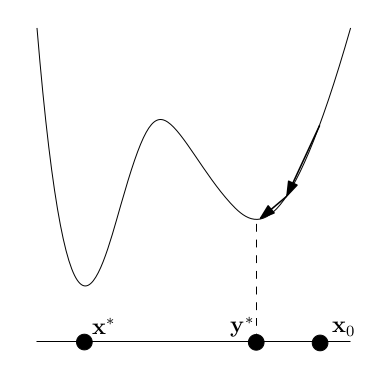
\includegraphics[width=0.5\columnwidth]{figures/non_convex}
	\label{fig:figures-non_convex}
\end{figure}
Main problem, is that we may get stuck in a local minimum, or in a saddle point, or run off to infinity,\ldots
\begin{figure}[htpb]
	\centering
	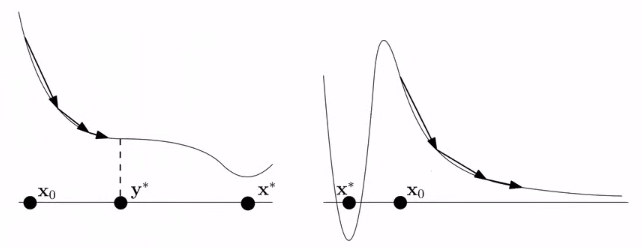
\includegraphics[width=0.9\columnwidth]{figures/non_convex_2}
	\label{fig:figures-non_convex_2}
\end{figure}

\defentry[Smoothness] Interestingly, smoothness doesn't require convexity, so we can use it even with non-convex functions.
\defentry[Convave] $f$ is concave is $-f$ is convex (for all $\mathbf{x}$, $f$ is below the tangent  at $x$).

\defentry[Bounded Hessians]
\begin{lemma*}
	Let $f: \dom(f) \to \R$ be twice differentiable, with $X \subset \dom(f)$ a convex set, and $\|\nabla^2 f(\mathbf{x})\| \leq L$ for all $\mathbf{x}\in X$, where $\|\cdot \|$ is the spectral norm. Then $f$ is smooth with parameter $L$ over $X$.
\end{lemma*}
So bounded Hessians $\Rightarrow$ smooth. The opposite (smooth $\Rightarrow$ bounded Hessians) is true over any open convex set $X$.

\defentry[Convergence]	We sadly can't prove that we will converge to $x^\star$. But we can show that we will converge to a null gradient, at the same rate that we converge to $x^\star$ in the convex case (for $t \to \infty$ ). This implies that we may converge to a saddle point, or we are following an asymptote ($e^{-x}$ will converge after infinite steps).
\defentry[Smooth] (but not necessarily convex). For $f$ smooth with parameter $L$, and with stepsize $\gamma := \frac{1}{L}$, GD yields \[
	\frac{1}{T}\sum_{t=0}^{T-1}\|\nabla f(\mathbf{x}_t)\|^2 \leq \frac{2L}{T}\left( f(\mathbf{x}_0) - f(\mathbf{x}^\star) \right)
\]
Note that we now have information on the average of the squared gradients, and not the actual values.
\defentry[No overshooting] If the function is smooth, and with the stepsize 1/L, gradient cannot overshoot (i.e. pass a critical point).

\defentry[Trajectory analysis] For  non-convex functions, it's nice to have a good starting point and what happens when we start there.

\defentry[Linear models with many outputs] We have $n$ data points, meaning $n$ inputs $x_i \in \R^d$ and $n$ outputs $y_n \in \R$. Hypothesis: $y_i \approx \mathbf{w}^\top x_i$ for some weight vector $\mathbf{w} \in \R^d$. We can generalize to more than one output value for each data point: $n$ outputs $\mathbf{x}_n \in \R^m$. Hypothesis: $\mathbf{y}_i \approx W\mathbf{x}_i$ for a weight \textit{matrix} $W \in \R^{m \times d}$.

\defentry[Minimize LS] To find that matrix $W^\star$ we pick the one that minimizes the least-squares error when taking into account all data points: \[
	W^\star = \argmin_{W \in \R^{m\times d}}\sum_{i=1}^{n} \|W \mathbf{x}_i - \mathbf{y}_i\|^2
\]
Notation:
\begin{itemize}
	\item $X \in \R^{d\times n}$: columns are the $\mathbf{x}_i$
	\item $Y \in \R^{m\times n}$: columns are the $\mathbf{y}_i$
\end{itemize}
This makes equivalent to compute \[
	W^\star = \argmin_{W \in \R^{m\times d}} \|WX - Y\|^2_F
\]
This is cool for us: this argmin is a linear transformation $f(W)$. With that, the optimal is when the gradient is 0: $\nabla f(W^\star) = \mathbf{0}$. Equivalent to training a linear neural network with one layer under LS error.

\defentry[Deep Linear NN] Even with several layers ($W_1, W_2, W_3$), as long as the composition is linear, we can concatenate to $\mathbf{y}= W\mathbf{x},\ W := W_3W_2w_1$.
\begin{figure}[htpb]
	\centering
	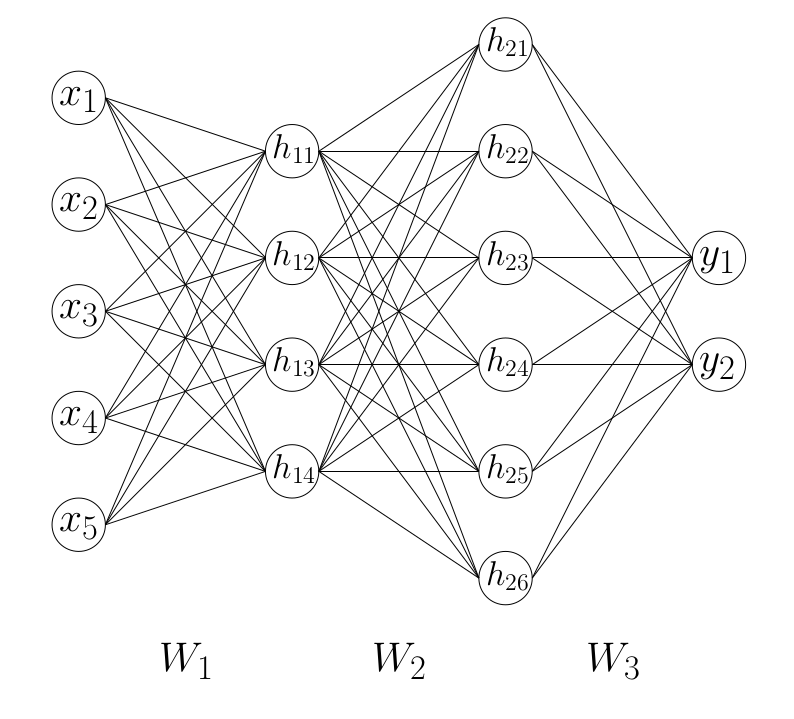
\includegraphics[width=0.9\columnwidth]{figures/linear_nn}
	\caption{Multi-layers linear NN}
	\label{fig:linear-nn}
\end{figure}

Training with $\ell$ layers: \[
	W^\star = \argmin_{W_1,W_2,\ldots,W_\ell} \|\underbrace{W_\ell W_{\ell-1}\cdots W_1X}_{\text{Prediction}} - \overbrace{Y}^{\text{Output}}\|^2_F
\]
From here, we use a toy example: all matrices are $1 \times 1$, $W_i = x_i, X=1, Y=1, \ell=d$, so $f: \R^d \to  \R$.\[
	f(\mathbf{x}) := \frac{1}{2} \left( \prod_{k=1}^{d} x_k -1 \right)^2
\]
\defentry[Gradient] With this toy $f$, the gradient is the following: \[
	\nabla f(\mathbf{x} = \left( \prod_k x_k -1 \right) \left( \prod_{k \neq 1}^{} ,\ldots,\prod_{k\neq d}^{} x_k   \right) .
\]

\defentry[Convergence analysis] We want to show that for any  $d > 1$ and from anywhere in $X : \left\{ \mathbf{x}: \mathbf{x} > \mathbf{0},  \prod_{k} \mathbf{x}_k \le 1 \right\}$, gradient descent will converge to a global minimum. $f$ is not smooth over $X$, but we can show that it is smooth along the trajectory of the gradient for suitable $L$, so that we get sufficient decrease \[
	f(\mathbf{x}_{t+1}) \le  f(\mathbf{x}_t) - \frac{1}{2L}\|\nabla f(\mathbf{x}_t)\|^2,\ t \ge  0
\]
So we can't converge to a saddle point. For $\mathbf{x} > \mathbf{0}, \prod_k \mathbf{x}_k \ge 1$, we also get convergence. But there are also starting points from which gradient descent will not converge to a global minimum.

\defentry[Balanced iterates] Let $\mathbf{x} > \mathbf{0}$ (component wise) and let $c \geq 1$ be a real number. $\mathbf{x}$ is called $c-balanced$ if $x_i \leq cx_j$ for all $1\leq i,j \leq d$.
\begin{lemma*}
	Let $\mathbf{x} \geq \mathbf{0}$ be c-balanced with $\prod_k x_k \leq 1$. Then for any stepsize $\gamma > 0$, $\mathbf{x}' := \mathbf{x} - \gamma \nabla f(\mathbf{x})$ satisfies $\mathbf{x}' \geq \mathbf{x}$ (componentwise) and is also c-balanced.
\end{lemma*}

\defentry[Bounded Hessians] We start by computing the Hessian: \[
	\nabla^2 f(\mathbf{x})_{ij} = \left\{
	\begin{array}{ll}
		\left(\prod\limits_{k \neq i} x_k \right)^2                                                & j=i       \\
		2 \prod\limits_{k \neq i}x_k \prod\limits_{k \neq  j} x_k - \prod\limits_{k \neq  i,j} x_k & j \neq  i
	\end{array}
	\right\}
\]
\begin{lemma*}
	Suppose that $\mathbf{x} > \mathbf{0}$ is c-balanced. Then for any $I \subseteq \{1,\ldots,d\}$, we have \[
		\left( \frac{1}{c} \right)^{|I|} \left( \prod\limits_k x_k \right)^{1- \frac{|I|}{d} } \leq  \prod\limits_{k \not\in I} x_k \leq  c^{|I|} \left( \prod\limits_k x_k \right)^{1-\frac{|I|}{d}}
	\]
\end{lemma*}

\begin{lemma*}
	Let $\mathbf{x} > \mathbf{0}$ be c-balanced with $\prod_k x_k \le  1$. Then \[
		\|\nabla^2f(\mathbf{x})\| \le  \|\nabla^2 f(\mathbf{x})\|_F \le  3dc^2
	\]
	Where $\|\cdot \|$ is the spectral norm, and $\|\cdot \|_F$ is the Frobenius norm.
\end{lemma*}

\defentry[Smoothness along the trajectory]
\begin{lemma*}
	Let $\mathbf{x} > \mathbf{0}$ be c-balanced, with $\prod_k x_k < 1,\ L = 3dc^2$. Let $\gamma := \frac{1}{L}$. Then for all $0 \ge \nu \ge  \gamma$, \[
		\mathbf{x}' := \mathbf{x} - \nu \nabla f(\mathbf{x}) \ge  \mathbf{x}
	\]
	is c-balanced with $\prod_k x_k' \le  1$, and $f$ is smooth with parameter $L$ over the line segment connecting $\mathbf{x}$ and $\mathbf{x} - \gamma \nabla f(\mathbf{x})$.
\end{lemma*}

\defentry[Convergence]
\begin{theorem*}
	Let $c \ge 1$ and $\delta > 0$ such that $\mathbf{x}_0 > \mathbf{0}$ is c-balanced with $delta \leq \prod_k(\mathbf{x}_0)_k < 1$. Choosing stepsize $\gamma = \frac{1}{3dc^2}$, gradient descent satisfies \[
		f(\mathbf{x}_T) \le \left( 1- \frac{\delta^2}{3c^{4}} \right)^{T} f(\mathbf{x}_0),\ T \ge 0
	\]
\end{theorem*}

\section{Accelerated Gradient Descent}
\defentry[Idea] On smooth functions, gradient descent is good but perhaps not as fast as it could be. Don't forget it's just some algorithm that uses gradient information, perhaps there is a better first-order method for smooth convex functions with a smaller upper-bound on the number of gradients computed.
\begin{theorem*}
	Every first-order method needs in the worst case $\Gamma/\sqrt{\epsilon}$ steps (gradients evaluations) in order to achieve an additive error of $\epsilon$ on smooth functions.
\end{theorem*}
There is a gap between $\O(1/\epsilon)$ (gradient descent) and the lower bound!

\defentry[Nesterov's accelerated GD] Let $f: \R^d \to \R$ be convex, differentiable and smooth with parameter $L$, Choose $\mathbf{z}_z = \mathbf{y}_0 = \mathbf{x}_0$ arbitrary. For $t \ge 0$, set \[
	\begin{array}{lll}
		\mathbf{y}_{t+1} & := & \mathbf{x}_t - \frac{1}{L}\nabla f(\mathbf{x}_t)                \\
		\mathbf{z}_{t+}  & := & \mathbf{z}_z - \frac{t+1}{2L} \nabla f(\mathbf{x}_t)            \\
		\mathbf{x}_{t+1} & := & \frac{t+1}{t+3}\mathbf{y}_{t+1} + \frac{2}{t+3}\mathbf{z}_{t+1}
	\end{array}
\]
Perform a ``smooth step'' from $\mathbf{x}_t$ to $\mathbf{y}_{t+1}$, then perform a more aggressive step from $\mathbf{z}_t$ to $\mathbf{z}_{t+1}$. Next iterate, $\mathbf{x}_{t+1}$ is a weighted average of $\mathbf{y}_{t+1}$ and $\mathbf{z}_{t+1}$, where we compensate for the more aggressive step by giving $\mathbf{z}_{t+1}$ a relatively low weight.

\defentry[Error bound]
\begin{theorem*}
	Let $f: \R^d \to  \R$ be convex and differentiable with a global minimum $\mathbf{x}^\star$; furthermore, suppose that $f$ is smooth with parameter $L$. Accelerated gradient descent yields \[
		f(\mathbf{y}_T) - f(\mathbf{x}^\star) \le \frac{2L \|\mathbf{z}_0 - \mathbf{x}^\star\|^2}{T(T+1)},\ T > 0
	\]
\end{theorem*}
To reach error at most $\epsilon$, accelerated gradient descent therefore only needs $\O(1/\sqrt{\epsilon})$ steps instead of $\O(1/\epsilon)$. Recall the bound for gradient descent: \[
	f(\mathbf{x}_T) - f(\mathbf{x}^\star) \le  \frac{L}{2T} \|\mathbf{x}_0 - \mathbf{x}^\star\|^2, T > 0
\]
\defentry[Potential function] Idea: assign a potential $\Phi(T)$ to each time  $t$ and show that $\Phi(t+1) \le  \Phi(t)$. We define the potential as \[
	\Phi(t) := t(t+1)(f(\mathbf{y}_t) - f(\mathbf{x}^\star)) + 2L \|\mathbf{z}_t - \mathbf{x}^\star\|^2
\]
If we can show that the potential always decrease, we get $\Phi(T) \le  \Phi(0)$, and replacing + rewriting we get the claimed error bound.

\section{Newton's Method}
\defentry[1D Case] Also called the \textit{Newton-Raphson Method}. The goal is to find a zero of a differentiable $f: \R \to \R$. Method: \[
	\begin{array}{l}
		x_{t+1} := x_t - \frac{f(x_t)}{f'(x_t)}, t \ge 0 \\
		f(x_t) + f'(x_t)(x-x_t) = 0
	\end{array}
\]
\begin{figure}[htpb]
	\centering
	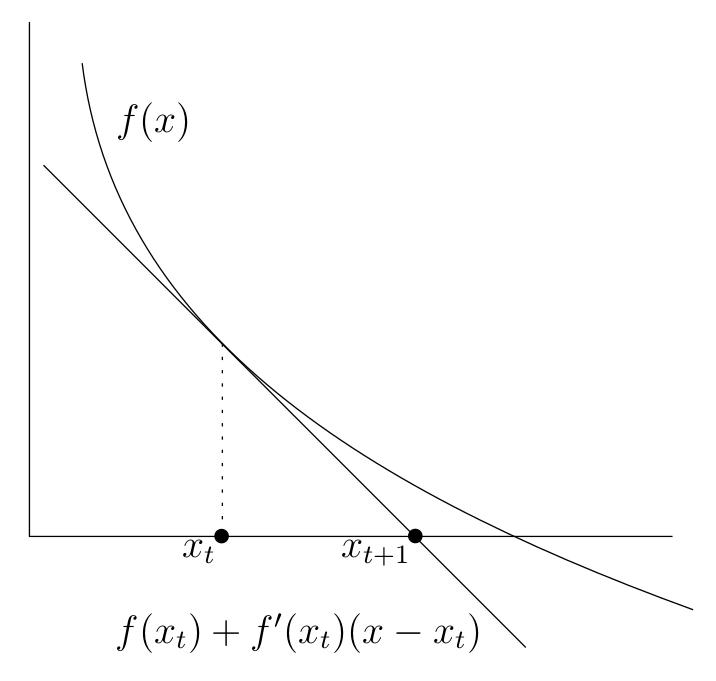
\includegraphics[width=0.8\columnwidth]{figures/newton_1d}
	\caption{Newton-Raphson Method}
	\label{fig:newton-raphson-1d}
\end{figure}
Illustration is at figure \ref{fig:newton-raphson-1d}
\defentry[Newton's Method for optim] \textbf{1D Case}: find a global minimum $x^\star$ of a differentiable function $f: \R \to \R$. Can equivalently search for a zero of the derivative $f'$ : apply the Newton-Raphson method to $f'$. Note that requires $f$ twice differentiable. Update step: \[
	x_{t+1} := x_t - \frac{f'(x_t)}{f''(x_t)} = x_t - f''(x_t)^{-1}f'(x_t)
\]
\textbf{d-dimensional case}: Newton's method for minimizing a convex function $f: \R^d \to \R$: \[
	\mathbf{x}_{t+1} := \mathbf{x}_t - \nabla^2f(\mathbf{x}_t)^{-1}\nabla f(\mathbf{x}_t)
\]
\defentry[Newton as adaptive GD] In general, the update for first order method is as follow: $\mathbf{x}_{t+1} =\mathbf{x}_t - H(\mathbf{x}_t) \nabla f(\mathbf{x}_t)$, with $H(\mathbf{x}) \in \R^{d\times d}$ is some matrix. For regular GD, $H = \gamma I$, while for newton we have $H = \nabla^2f(\mathbf{x}_t)^{-1}$. Thus Newton's method is an ``adaptive gradient descent'', adaptation is w.r.t the local geometry of the function at $\mathbf{x}_t$.

\defentry[Nondegenerate quadratic function] A nondegenerate quadratic function is of the form \[
	f(\mathbf{x}) = \frac{1}{2}\mathbf{x}^\top M\mathbf{x} - \mathbf{q}^\top \mathbf{x} + c
\]
Where $M \in \R^{d\times d}$ is an invertible symmetric matrix, $\mathbf{q} \in  \R^d$, $c \in \R$. Let $\mathbf{x}^\star = M^{-1}\mathbf{q}$ be the unique solution of $\nabla f(\mathbf{x}) = \mathbf{0}$. $\mathbf{x}^\star$ is the unique global minimum if $f$ is convex.
\begin{lemma*}
	On nondegenerate quadratic functions, any starting point $\mathbf{x}_0 \in \R^d$, Newton's method yields $\mathbf{x}_1 = \mathbf{x}^\star$.
\end{lemma*}


\defentry[Affine Invariance] Newton's method is affine invariant (invariant under any invertible affine transformation).
\begin{figure}[htpb]
	\centering
	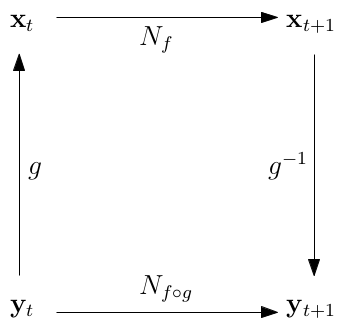
\includegraphics[width=0.8\columnwidth]{figures/affine_invariance}
	\caption{Affine Invariance}
	\label{fig:affine-invariance}
\end{figure}
\begin{lemma*}
	let $f: \R^d \to \R$ be twice differentiable, $A \in \R^{d\times d}$ an invertible matrix, $\mathbf{b} \in \R^d$. Let $g: \R^d \to \R$ be the (bijective) affine function $g(\mathbf{y}) = A\mathbf{y} + \mathbf{b},\ \mathbf{y} \in \R^d$. Finally, for a twice differentiable function $h: \R^d \to \R$, let $N_h: \R^d \to \R^d$ denote the Newton step for $h$, i.e. \[
		N_h(\mathbf{x}) = \mathbf{x} - \nabla^2 h(\mathbf{x})^{-1}\nabla h(\mathbf{x})
	\]
	whenever this is defined. Then we have $N_{f \circ g} = g^{-1} \circ N_f \circ g$.
\end{lemma*}

\defentry[Newton as Taylor] Alternatively, we can interpret each step as minimizing the local second-order Taylor approximation
\begin{lemma*}
	Let $f$ be convex and twice differentiable at $\mathbf{x}_t \in \dom(f)$, with $\nabla^2 f(\mathbf{x}_t) \succeq 0$ being invertible. The vector $\mathbf{x}_{t+1}$ resulting from the Newton step satisfies \[
		\begin{array}{ll}
			\mathbf{x}_{t+1} = \argmin_{\mathbf{x} \in \R^d} & f(\mathbf{x}_t) \\&+ \nabla f(\mathbf{x}_t)^\top (\mathbf{x} - \mathbf{x}_t) \\& + \frac{1}{2} (\mathbf{x} - \mathbf{x}_t)^\top \nabla^2 f(\mathbf{x}_t)(\mathbf{x}-\mathbf{x}_t)
		\end{array}
	\]
\end{lemma*}

\defentry[Local convergence] Under suitable conditions, and starting close to the global minimum, Newton's method will reach distance at most $\epsilon$ to the minimum within $\log \log (1/\epsilon)$ steps. Much faster, but we need to start close to the minimum already. This is a local convergence result.

\textbf{[\ldots missing]} %TODO

\defentry[Downsides] We have a computational bottleneck in each step: we need to either compute and invert the Hessian matrix, or solve the linear system $\nabla^2 f(\mathbf{x}_t) \Delta \mathbf{x} = -\nabla f(\mathbf{x}_t)$ for the next step $\Delta \mathbf{x}$. Matrix/system has size $d\times d$, taking up to  $\O(d^3)$ time to invert/solve, while $d$ may be large.

\defentry[The secant method] Yet another iterative method for finding zeros in dimension 1. Now, use finite difference approximation: $f'(x_t) \simeq \frac{f(x_t) - f(x_{t-1})}{x_t - x_{t-1}}$ \footnote{for $|x_t - x_{t-1}$ | small}, and replace in Newton-Raphson step to have the secant method.

This is nice, because this is a derivative-free version of the Newton-Raphson method. We can also optimize a differentiable univariate function $f$, by applying the secant method to $f'$. \[
	x_{t+1} := x_t - f'(x_t) \frac{x_t - x_{t-1}}{f'(x_t) - f'(x_{t-1)}}
\]

\defentry[Secant in high dim] Possible if we match the \textbf{the secant condition} %TODO
\defentry[Quasi-newton methods] %TODO

\section{Frank-Wolfe}
\defentry[Intro] An alternative algorithm to optimize smooth convex function over compact set. The main difference with the projected gradient descent is that it doesn't require a projection step, which can be quite costly.
\defentry[Algorithm] \[
	\begin{array}{l}
		\mathbf{s}:= LMO(\nabla f(\mathbf{x}_t)), \\
		\mathbf{x}_{t+1} := (1-\gamma) \mathbf{x}_t +  \gamma \mathbf{s}
	\end{array}
\]
For time steps $t = 0,1,\ldots,$ and stepsize $\gamma := \frac{2}{t+2}$. We also define LMO (Linear Minimization Oracle) as a scalar product: \[
	LMO(\mathbf{g}) := \argmin_{\mathbf{s} \in X}  \left< \mathbf{s}, \mathbf{g} \right>
\]
\defentry[Properties]
\begin{itemize}
	\item Always feasible (implies $\mathbf{x}_0, \mathbf{x}_1,\ldots,\mathbf{x}_t \in X$). Because $\mathbf{x}_{t+1}$ is on line segment $\left[ \mathbf{s}, \mathbf{x}_t \right] $ for $\gamma \in \left[ 0,1 \right] $.
	\item Reduces non-linear to linear optimization.
	\item Projection-free
	\item Sparse iterates (in terms of corners $\mathbf{s}$ used). At most, one extreme point is added at each step!
\end{itemize}
\defentry[Frank-Wolfe and Lasso] The each step has complexity $\O(d)$, much better than projected gradient descent.
\defentry[Duality Gap] \[
	g(\mathbf{x}) := \left< \mathbf{x}-\mathbf{s}, \nabla f(\mathbf{x})\right>
\] This gives a certificate for optimization quality: \[
	\begin{array}{ll}
		g(\mathbf{x}) & = \max\limits_{\mathbf{s} \in X}\left<\mathbf{x}-\mathbf{s}, \nabla f(\mathbf{x}) \right> \\
		              & \ge \left<\mathbf{x}-\mathbf{a}^\star, \nabla f(\mathbf{x}) \right>                       \\
		              & \ge f(\mathbf{x}) - f(\mathbf{x}^\star)
	\end{array}
\]
\defentry[Stepsize variants] \[
	\begin{array}{lllr}
		\gamma   & := & \frac{2}{t+2}                                                                                                             \\
		\gamma_t & := & \argmin\limits_{\gamma \in \left[ 0,1 \right]} f\big((1-\gamma)\mathbf{x}_t + \gamma \mathbf{s}\big) & \text{line search} \\
		\gamma_t & := & \min \left\{ \frac{g(\mathbf{x}_t)}{L \|\mathbf{s} - \mathbf{x}\|^2}, 1 \right\}                     & \text{gap-based}
	\end{array}
\]
\defentry[Convergence]
\begin{theorem*}
	Let $f: \R^d \to \R$ be convex and smooth with parameter L, and $\mathbf{x}_0 \in X$. Then choosing any of the above stepsizes, the Frank-Wolfe algorithm yields \[
		f(\mathbf{x}_T) - f(\mathbf{x}^\star) \le \frac{2L\text{diam}(X)^2}{T+1}
	\]
	Where $\text{diam}(X) := \max_{\mathbf{x},\mathbf{y} \in X} \|\mathbf{x}-\mathbf{y}\|$ is the diameter of $X$.
\end{theorem*}
We then have a convergence of rate $\O(\frac{L}{T})$, which is the same as PGD. It's also suboptimal, compared to accelerated GD (with rate of $\O(\frac{L}{T^2})$. The proof uses the following lemma:
\begin{lemma*}
	For a step $\mathbf{x}_{t+1} := \mathbf{x}_t + \gamma(\mathbf{s}-\mathbf{x}_t)$ with an arbitrary step-size $\gamma \in \left[ 0,1 \right] $, it holds that \[
		f(\mathbf{x}_{t+1} \le f(\mathbf{x}_t) - \gamma g(\mathbf{x}_t) + \frac{\gamma^2}{2}L\text{diam}(X)^2
	\] if $\mathbf{s} = LMO(\nabla f(\mathbf{x}_t))$.
\end{lemma*}

\defentry[Curvature constant] We define the constant $C_f$ as \[
	\sup_{\substack{\mathbf{x},\mathbf{s} \in X, \gamma \in \left[ 0,1 \right] \\ \mathbf{y}=\mathbf{x}+\gamma(\mathbf{s}-\mathbf{x})}} \frac{2}{\gamma^2} (f(\mathbf{y}) - f(\mathbf{x}) - \left<\mathbf{y}-\mathbf{x},\nabla f(\mathbf{x}) \right>)
\]
\defentry[Affine invariance] The algorithm is invariant to scaling (affine transformations) of the input problem. And so is $C_f$.
\defentry[Convergence in Duality Gap]
\begin{theorem*}
	Let $f: \R^d \to \R$ be convex and smooth with parameter L, and $\mathbf{x}_0 \in X$, $T \ge 2$. Then choosing any of the above stepsizes, the Fran-Wolfe algorithm yields a $t,\ 1 \le  t \le T$ such that \[
		g(\mathbf{x}_t) \le \frac{27/4 C_f}{T+1}
	\]
\end{theorem*}

\section{Coordinate Descent}
\defentry[Idea] This is yet another first-order optimization method. As before, we look for $x^\star \in \R^d$, by minimizing $f(\mathbf{x})$. We do so by updating one coordinate at a time, while keeping the other fixed. By definition, the value will decrease at each step.
\defentry[Algorithm] At time $t$, select a coordinate $i_t \in \left[ d \right] $, then compute $\mathbf{x}_{t+1} := \mathbf{x}_t + \gamma \mathbf{e}_{i_t}$. From that, you have 2 variants: either a gradient-based step-size $\big(\mathbf{x}_{t+1} := \mathbf{x}_t - \frac{1}{L}\nabla_{i_t} f(\mathbf{x}_t) \mathbf{e}_{i_t}\big)$, or by exact coordinate minimization (solve the single-variable minimization $\argmin_{\gamma \in \R} f(\mathbf{x}_t + \gamma \mathbf{e}_{i_t})$ ). The latter is easy to solve, can be approximately solved, and has no hyperparameter to tune.
\defentry[Randomized Coordinate Descent] We first select the index $i_t \in \left[ d \right] $ uniformly at random, then compute the next step  \[
	\mathbf{x}_{t+1} := \mathbf{x}_t - \frac{1}{L} \nabla_{i_t} f(\mathbf{x}_t) \mathbf{e}_{i_t}
\]
\defentry[Convergence] We assume coordinate-wise smoothness. It is equivalent to coordinate-wise Lipschitz-gradient. Additionally, we assume strong convexity ($\mu > 0$).
\begin{theorem*}
	Let $f$ be coordinate-wise smooth with constant $L$, and strongly convex with parameter $\mu > 0$. Then, coordinate descent with a step-size of $\frac{1}{L}$ (as above) when choosing the active coordinate $i_t$ uniformly at random, has an expected linear convergence rate of \[
		\E\left[f(\mathbf{x}_t) - f^\star\right] \le \left( 1- \frac{\mu}{dL} \right)^t \left[ f(\mathbf{x}_0) - f^\star \right] .
	\]
\end{theorem*}
\defentry[The Polyak-Lojasiewicz Condition]
\begin{definition*}
	$f$ satisfies the PL inequality if the following holds for some $\mu > 0$ : \[
		\frac{1}{2} \|\nabla f(\mathbf{x})\} \|^2 \ge  \mu(f(\mathbf{x}) - f^\star),\ \forall \mathbf{x}
	\]
\end{definition*}
\begin{lemma*}
	Strong convexity $\to $ PL. Let $f$ be strongly convex, with parameter $\mu > 0$. Then $f$ satisfies PL for the same $\mu$.
\end{lemma*}

\defentry[Importance Sampling] Uniformly random selection is not always the best. For that, we define individual smoothness constants $L_i$ for each coordinate $i$ : \[
	f(\mathbf{x} + \gamma \mathbf{e}_i) \le f(\mathbf{x}) + \gamma \nabla_i f(\mathbf{x}) + \frac{L_i}{2}\gamma^2
\]
With these constants, we can define a biased sampling: $P\left[i_t = i\right] = \frac{L_i}{\sum_{i} L_i} $, and using a step-size of $\frac{1}{L_{i_t}}$, this converges with a faster rate of \[
	\E\left[f(\mathbf{x}_t) - f^\star\right] \le \left( 1 - \frac{\mu}{d \bar{L}} \right)^t \left[ f(\mathbf{x}_0) - f^\star \right]
\]
With $\overline{L}$ the mean of $L_i$

\defentry[Steepest coordinate descent] Other coordinate selection rule:  $i_t := \argmax_{i \in \left[ d \right] } |\nabla_i f(\mathbf{x}_t)|$. This is a greedy algorithm. It now becomes deterministic, and not random anymore. Same convergence rate as for random coordinate descent.
\defentry[Faster convergence with steepest] A faster convergence can be obtained when the strong convexity f $f$ is measured with respect to the $\ell_1$-norm instead of the normal Euclidean norm, i.e. \[
	f(\mathbf{y}) \ge f(\mathbf{x}) + \left<\nabla f(\mathbf{x}), \mathbf{y}-\mathbf{x} \right> + \frac{\mu_1}{2} \|\mathbf{y}-\mathbf{x}\|^2_{1}.
\]
If $f$ is coordinate-wise $L$-smooth, strongly convex w.r.t the $\ell_1$-norm with parameter $\mu_1$ > 0, and step-size of $\frac{1}{L}$, we have a linear convergence rate of  \[
	\left[f(\mathbf{x}_t) - f^\star\right] \le \left( 1-\frac{\mu_1}{L} \right)^t \left[ f(\mathbf{x}_0) - f^\star \right]
\]
\defentry[Non-Smooth] For general non-smooth $f$, coordinate descent fails (gets permanently stuck). But if the non-smooth part is separable over the coordinates, we have global convergence. This means \[
	f(\mathbf{x}) := g(\mathbf{x}) + h(\mathbf{x}),\ h(\mathbf{x}) = \sum_i h_i(x_i)
\]
(e.g. $f(\mathbf{x}) := \|\mathbf{x}\|^2 + \|\mathbf{x}\|_1$)

\subsection{Duality}
\defentry[Conjugate] Given a function $f: \R^d \to  \R^+$, the conjugate $f^*: \R^d \to \R^+$ is defined as  \[
	f^*(\mathbf{y}) := \max_\mathbf{x}\ \mathbf{x}^\top \mathbf{y} - f(\mathbf{x})
\]
Also called \textit{Legendre transform} or \textit{Fenchel conjugate function}. Note that $\R^+ := \R \cup \left\{ +\infty \right\} $.
\begin{figure}[htpb]
	\centering
	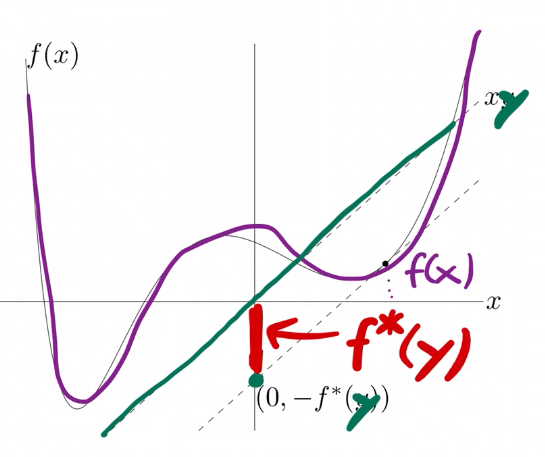
\includegraphics[width=0.8\columnwidth]{figures/duality_gap}
	\caption{Maximum gap}
	\label{fig:duality_gap}
\end{figure}
Here is another way of looking at it: given $\mathbf{y}$, draw the slope line (green). Then look at the point of $f(\mathbf{x})$ that is the \textit{furthest below} (it's not an absolutes difference). This can also be achieved by taking the parallel to the slope, and evaluating at $\mathbf{x} = \mathbf{0}$.
\defentry[Properties of conjugate]
\begin{itemize}
	\item $f^*$ is always convex, even if $f$ is not.
	\item \textit{Fenchel's inequality}: \[
		      f(\mathbf{x}) + f^*(\mathbf{y}) \ge \mathbf{x}^\top \mathbf{y},\ \forall \mathbf{x},\mathbf{y}
	      \]
	\item Hence, the conjugate of the conjugate $f^{**}$ satisfies $f^{**} \le f$. The second conjugate is also convex, and can be interpreted as the ``envelope'' of the original function.
	\item If $f$ is closed an convex, then $f^{**} = f$
	\item if if closed and convex, then for any $\mathbf{x},\mathbf{y}$ : \[
		      \begin{array}{ll}
			      \mathbf{y} \in \partial f(\mathbf{x}) & \Leftrightarrow \mathbf{x}\in \partial f^*(\mathbf{y})                       \\
			                                            & \Leftrightarrow f(\mathbf{x}) + f^*(\mathbf{y}) = \mathbf{x}^\top \mathbf{y}
		      \end{array}
	      \]
	\item Separable functions: if $f(\mathbf{u},\mathbf{v}) = f_1(\mathbf{u}) + f_2(\mathbf{v})$, then $f^*(\mathbf{w},\mathbf{z}) = f^*_1(\mathbf{w}) + f^*_2(\mathbf{z})$
\end{itemize}

\defentry[Some known conjugates]
\begin{itemize}
	\item \textbf{Indicator function} of a set $C \subseteq \R^d$ \[
		      \indic_C(\mathbf{x}) := \left\{
		      \begin{array}{ll}
			      0       & \mathbf{x} \in C, \\
			      +\infty & \text{otherwise}.
		      \end{array}
		      \right.
	      \]
	      If $f(\mathbf{x}) = \indic_C(\mathbf{x})$, then the conjugate is \[
		      f^*(\mathbf{y}) = \max_{\mathbf{x}\in C}\mathbf{y}^\top \mathbf{x}
	      \]
	\item \textbf{Norm}: if $f(\mathbf{x}) = \|\mathbf{x}\|$, then its conjugate is \[
		      f^*(\mathbf{y}) = \indic_{\left\{ \mathbf{z}: \|\mathbf{z}\|_* \le 1 \right\} }(\mathbf{y})
	      \]
	      Which corresponds to the indicator of the dual norm ball. Note: the dual norm of $\|.\|$ is defined as $\|\mathbf{y}\|_* := \max_{\|\mathbf{x}\| \le 1} \mathbf{y}^\top - \mathbf{x}$. E.g. $\|.\|_1 \leftrightarrow \|.\|_{\infty}$
  \item \textbf{Generalized linear models} $\min_{\mathbf{x}\in \R^d} f(A\mathbf{x}) + g(\mathbf{x})$. We reformulate as $\min_{\mathbf{x} \in \R^d, \mathbf{w} \in \R^n} f(\mathbf{w}) + g(\mathbf{x})$, such that $\mathbf{w} = A\mathbf{x}$. We define the Lagrange dual function: \[
				  \begin{array}{ll}
						  \mathcal{L}(\mathbf{u}) & := \min\limits_{\substack{\mathbf{x}\in \R^d\\ \mathbf{w}\in \R^n}}f(\mathbf{w}) + g(\mathbf{x}) + \mathbf{u}^\top(\mathbf{w} - A\mathbf{x}) \\
				  &= -f^*(-\mathbf{u}) - g^*(A^\top\mathbf{u})
				 \end{array}
  \] 
  And thus, gives rise to the \textbf{dual problem}: minimizing the above function is the same as maximizing the conjugate : \[
		  \max\limits_{\mathbf{u}\in \R^n}\left[ \mathcal{L}(\mathbf{u}) = -f^*(-\mathbf{u}) - g^*(A^\top\mathbf{u}) \right] 
  \] 
  \item \textbf{Lasso} $\min\limits_{x \in \R^d} \frac{1}{2} \|A\mathbf{x} - \mathbf{b}\|^2 + \lambda \|\mathbf{x}\|_1$. We use separability to split the two as $f(\mathbf{w})$ and $g(\mathbf{x})$. This yields \[
				  \begin{array}{l}
						  f^*(\mathbf{u}) = \frac{1}{2} \|\mathbf{b}\|^2 - \frac{1}{2}\|\mathbf{b}- \mathbf{u}\|^2 \\
						  g^*(\mathbf{v}) = \indic_{\mathbf{z}:\|\mathbf{z}\|_{\infty} \le  1}(\mathbf{v}/\lambda)
  \end{array}
  \] 
  We then define the dual problem using the above function (GLM)

\end{itemize}

\defentry[Why duality] Duality gap gives a certificate of current optimization quality. The minimization of the former function is greater or equal to the maximization of the conjugate. The optimum value is then between those two. If they are close, we have a certificate of quality. You can then use the gap as a \textbf{stopping criterion}. And finally, in some cases, the dual can be easier to solve.

\subsection{Zero-order Optimization}
\defentry[Goal] Can we optimize without access to the gradient ?

\defentry[Random search] Pick a random direction $\mathbf{d}_t \in \R^d$. Define $\gamma := \argmin_{\gamma \in \R} f(\mathbf{x}_t + \gamma \mathbf{d}_t)$ (line-search). Finally, do a step: $\mathbf{x}_{t+1} := \mathbf{x}_t + \gamma \mathbf{d}_t$. \textit{Convergence} is the same as gradient descent, up to a slow-down factor $d$. For convex functions, we get a rate  $\O(dL/\epsilon)$, and for strongly convex we have $\O\left(dL\log(\frac{1}{\epsilon})\right)$


\defentry[Reinforcement Learning] State changes based on some inputs: $\mathbf{s}_{t+1} = f(\mathbf{s}_t, \mathbf{a}_t, \mathbf{e}_t)$, where $\mathbf{s}_t$ is the state of the system, $a_t$ is the control action and $\mathbf{e}_t$ is some random noise. We assume that $f$ is fixed, but unknown. We want to establish a policy based on previous actions and states: \[
		\mathbf{a}_t := \pi(\mathbf{a}_1,\ldots,\mathbf{a}_{t-1}, \mathbf{s}_0, \ldots,\mathbf{s}_t)
\] Which takes a trajectory of the dynamical system and outputs a new control action. The goal is to maximize the overall reward \[
\max\limits_{\mathbf{a}_t} \E_{\mathbf{e}_t}\left[ \sum_{t=0}^{N}R_t(\mathbf{s}_t, \mathbf{a}_t)  \right] 
\] using the definition of the next state ($\mathbf{s}_0$ given)

\subsection{Other SGD Methods}
\defentry[Adagrad] Adaptive variant of SGD:
\begin{enumerate}
		\item Pick a stochastic gradient $\mathbf{g}_t$ 
		\item update $\left[ G_t \right]_i := \sum_{s=0}^{t} \left( \left[ \mathbf{g}_s \right]_i \right)^2 $ 
		\item $\left[ \mathbf{x}_{t+1} \right]_i := [\mathbf{x}_t]_i - \frac{\gamma}{\sqrt{[G_t]_i} }[\mathbf{g}_t]_i$
\end{enumerate}
Standard choice for $\mathbf{g}_t := \nabla f_j(\mathbf{x}_t)$ four sum-structured objective functions $f = \sum_j f_j$. Normal SGD would skip step 2, and not divide $\gamma$ on step 3.

\defentry[Adam] Adam is a momentum variant of Adagram:
\begin{enumerate}
		\item pick a stochastic gradient $\mathbf{g}_t$ 
		\item $\mathbf{m}_t := \beta_1 \mathbf{m}_{t-1} + (1-\beta_1) \mathbf{g}_t$ (momentum term)
		\item $[\mathbf{v}_t]_i := \beta_2 [\mathbf{v}_{t-1}]_i + (1-\beta_2)([\mathbf{g}_s]_i)^2$ $\forall i$ (2nd order statistics
		\item $[\mathbf{x}_{t+1}]_i := [\mathbf{x}_t]_i - \frac{\gamma}{\sqrt{[\mathbf{v}_t]_i} } [\mathbf{m}_t]_i$ $\forall i$
\end{enumerate}
We now have an exponential decay. It's then faster at forgetting older weights. We have a momentum from previous gradients. There exists a simplified version without correction for initialization of $\mathbf{m}_0, \mathbf{v}_0$. In practice, we see strong performances e.g. for self-attention networks.

\defentry[SignSGD] Only use the sign (one bit) of each gradient entry. This is a communication efficient variant:
\begin{enumerate}
		\item Pick a stochastic gradient $\mathbf{g}_t$ 
		\item $[\mathbf{x}_{t+1}]_i := [\mathbf{x}_t]_i - \gamma_t sign([\mathbf{g}_t]_i)$ $\forall i$
\end{enumerate}
With possible rescaling of $\gamma_t$ with $\|\mathbf{g}_t\|_1$. This is communication efficient, for distributed training. But we face convergence issues.

\section{Otim for ML in practice}

%%%%%%%%%%%%%%%%%%
%%% APPENDIX %%%%%
%%%%%%%%%%%%%%%%%%
\newpage
\onecolumn
\appendix
\section{Tables and summaries}
\begin{table}[htpb]
	\centering
	\begin{tabular}{c|ccc}
		                           & GD                           & SGD                      & Sub-GD                     \\
		\hline
		Lipschitz convex           & $\O(\frac{1}{\epsilon^2})$   &                          & $\O(\frac{1}{\epsilon^2})$ \\
		Smooth \& convex           & $\O(\frac{1}{\epsilon})$                                                             \\
		Strongly convex            &                              & $\O(\frac{1}{\epsilon})$                              \\
		Smooth \& strongly  convex & $\O(\log\frac{1}{\epsilon})$
	\end{tabular}
	\caption{Convergence depending on function properties}
	\label{tab:convergence_speed}
\end{table}

\section{Useful functions}
\defentry[Euclidean Norm]  $\| X \|^2 = X^\top X = \sum_{n=1}^{d} x_i^2 \in \R_+$
\defentry[Triangle inequality] $\|\mathbf{x}+\mathbf{y}\| \le  \|\mathbf{x}\| + \|\mathbf{y}\|$
\defentry[Gradient] \[
	\nabla f(\mathbf{x}) := \left( \frac{\partial f}{\partial x_1} (\mathbf{x}),\ldots,\frac{\partial f}{\partial x_d} (\mathbf{x}) \right)
\]
\defentry[Hessian] \[
	\nabla^2 f(\mathbf{x}) = \begin{pmatrix}
		\frac{\partial^2 f}{\partial x_1 \partial x_1} (\mathbf{x}) & \frac{\partial^2 f}{\partial x_1 \partial x_2} (\mathbf{x}) & \cdots & \frac{\partial^2 f}{\partial x_1 \partial x_d} (\mathbf{x}) \\
		\frac{\partial^2 f}{\partial x_2 \partial x_1} (\mathbf{x}) & \frac{\partial^2 f}{\partial x_2 \partial x_2} (\mathbf{x}) & \cdots & \frac{\partial^2 f}{\partial x_2 \partial x_d} (\mathbf{x}) \\
		\vdots                                                      & \vdots                                                      & \cdots & \vdots                                                      \\
		\frac{\partial^2 f}{\partial x_d \partial x_1} (\mathbf{x}) & \frac{\partial^2 f}{\partial x_d \partial x_2} (\mathbf{x}) & \cdots & \frac{\partial^2 f}{\partial x_d \partial x_d} (\mathbf{x}) \\
	\end{pmatrix}
\]
\defentry[Positive semidefinite] A symmetric matrix $M$ is positive semidefinite if $\mathbf{x}^\top M\mathbf{x} \ge 0$ for all $\mathbf{x}$ and positive definite if $\mathbf{x}^\top M\mathbf{x} > 0$ for all $\mathbf{x}\neq \mathbf{0}$
\defentry[Spectral norm] Let $A$ be an $(m \times d)$-matrix. Then \[
	\|A\| := \max_{\mathbf{v} \in  \R^d, \mathbf{v} \neq 0} \frac{\|A\mathbf{v}\|}{\|\mathbf{v}\|} = \max_{\| \mathbf{v} \|=1} \|A\mathbf{v}\|
\] is the 2-norm (or spectral norm) of  $A$.
\defentry[Frobenius Norm] \[
	\|A\|_F = \sqrt{\sum\nolimits_{i,j} a^2_{ij}}
\]
Equivalent to the euclidean norm of $vec(A)$, the ``flattening'' of $A$.
\defentry[Scalar product] \[
	\left< \mathbf{s},\mathbf{g} \right> = \sum_{i} s_i g_i
\]
\end{document}

